\subsection{Chat}

The chat section of the application will be designed to resemble a standard chat interface such as the deign used for texting on cellphones. This means implementing features such as the sender and receiver having different colored messages, and opposite horizontal alignments for the messages from the sender and the receiver, which means messages will cling to each side of the chat window. This design choice was made to make the chatbot as accessible, familiar and easy to use as possible.
\Figureref{fig:chat_of_MathChatBot} shows a draft of the chat window in the application where you can see the layout of the messages.

\begin{figure}[H]
    \centering
    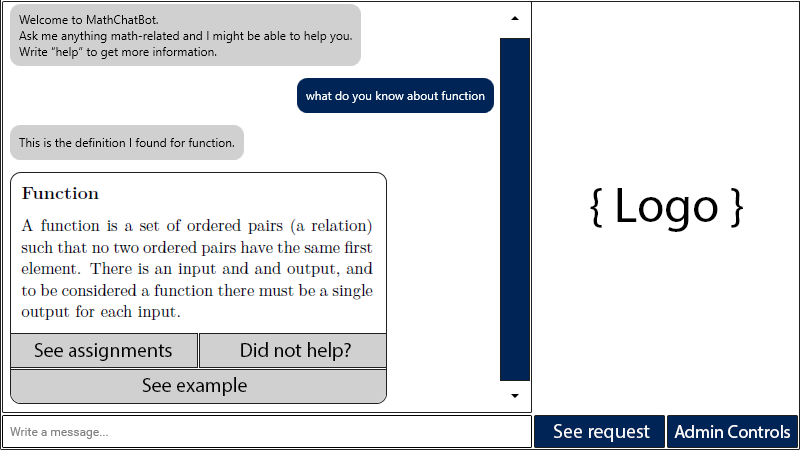
\includegraphics[width=0.6\textwidth]{figures/ChatDraft.png}
    \caption{Example of an entity analysis \cite{DemoAPI}}
    \label{fig:chat_of_MathChatBot}
\end{figure}

\noindent
As seen on \figureref{fig:chat_of_MathChatBot} the chatbot will include buttons when showing definitions, assignments and examples.
A topic definition will include the following buttons:

\begin{itemize}
    \item \textbf{See assignments}, shows assignments for each term related to the topic in question.
    \item \textbf{See terms}, gives a list of terms to the topic in question.
\end{itemize}

\noindent
\Figureref{fig:chat_of_MathChatBot} shows a draft of a term definition. This is the description of the buttons:

\begin{itemize}
    \item \textbf{See assignments}, shows assignments for the term in question.
    \item \textbf{See example}, shows examples for the term definition in question.
    \item \textbf{Did not help}, sends a help request for the term definition in question.
\end{itemize}



The buttons for the topic descriptions will include a \enquote{See assignments} button that will provide an assignment for the student regarding the topic asked for and a button named \enquote{See terms} which will provide a list of terms regarding the topic asked for. When accessing a specific term the user will be presented with 3 buttons. The first on being a \enquote{Did not help?} button that will register that the user has issues with a topic if pressed. A \enquote{See example} button that will give an example of how to use the term you asked the chatbot for. And the last button being a \enquote{See assignment} button which gives the user an assignment they can work with. Pressing this button will make the MathChatBot post an assignment with 2 buttons attached. The first one being a \enquote{See answers} which will give the student the answer for the assignment, and the second one being a \enquote{Need help?} button that has the same function as the previous mentioned \enquote{Did not help?} button. \newline

The figures used for the assignments and examples mentioned above are self-made. After a sketching of an example or assignment it would be saved and put into LaTeX with an accompanying text. Other Other options that using LaTeX have also been considered such as the program Word or a library named WPF-Math which is used for typing formulas into WPF. The idea of using Word was dismissed due to word not having an option for typing formulas in a professional-looking way while the library mentioned earlier which was made for typing out such formulas in WPF-Math did not have a feature for adding text which excluded the library as an option. As mentioned the the decision ended creating the needed material using LaTeX  because LaTeX made it possible to create both formulas and write text in a effective and professional-looking way.
